\documentclass[oneside, 10pt, notitlepage]{book}
	
	
\usepackage{../_mypackages/monographpreamble}
\usepackage{../_mypackages/commands}

\title{Special Relativity} % \MyTitle
\author{Bruno Murino} % \MyAuthor
\date{\today} % \MyDate

\usepackage{../_mypackages/monographstyle}

\graphicspath{ {figures/} }

%--------------------------------------------------------------------------------------------------

\begin{document}
\chapter{Lista XII}

\section*{Ex. 1)}

If we are on frame S and there's an isosceles triangle with sides \(l_a = l_b\) and \(l_c\), \(l_c > l\), there exists a frame \(S'\) which sees this triangles as equilateral. Lets find what should the speed of S' be so it sees the triangle as equilateral. The sides of the triangle on frame \(S'\) are \(l'_a=l'_b=l'_c\).

\begin{figure}[H]
    \centering
    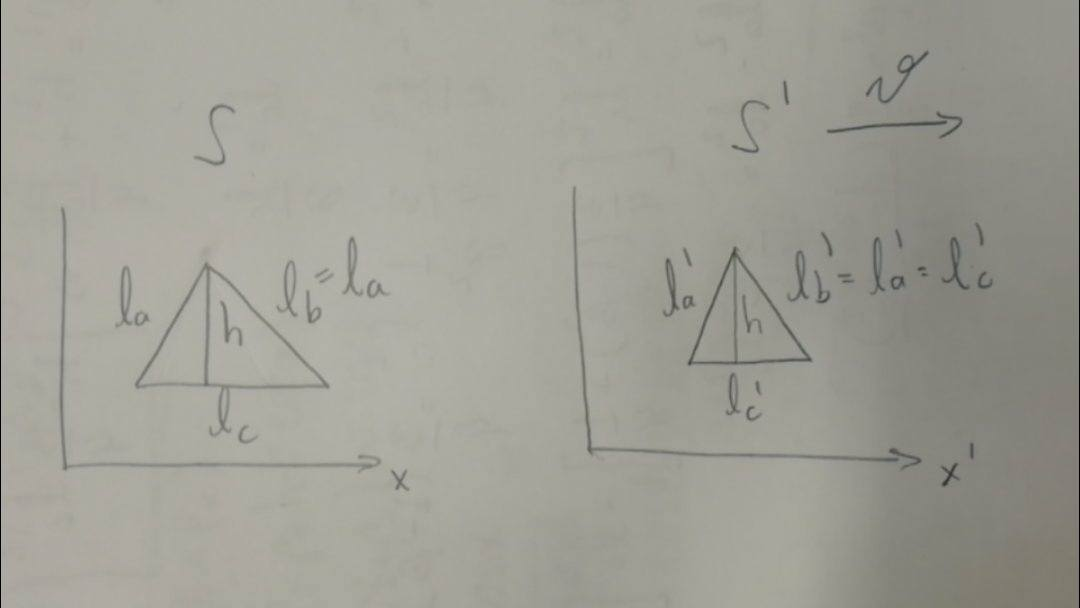
\includegraphics[width=0.7\textwidth]{L12_1}
    \label{fig:L12_1}
\end{figure}

First, lets place \(l_c\) along the \(x\)-axis and let \(S'\) move along the \(x\)-axis. Now we can conclude that the height of the triangle doesn't change, since it's perpendicular to the boost. Lets apply the Pythagorean theorem on the triangle whose sides are \(l_a\), \(h\) and \(l_c/2\) (frame \(S\)) and on the triangle whose sides are \(l_a'\), \(h\) and \(l'_c/2\) (frame \(S'\)). See figure \ref{fig:L12_1}. Thus
\begin{equation}\label{eq:A}
    l_a^2 = h^2 + \frac{1}{4}l^2_c
\end{equation}
\begin{equation}\label{eq:B}
    l'_a^2 = h^2 + \frac{1}{4}l'^2_c \qq{then} h^2= l'_a^2-\frac{1}{4}l'^2_c
\end{equation}
So, plugging \eqref{eq:B} onto \eqref{eq:A}, we find
\begin{equation}
    l_a^2 = l'_a^2-\frac{1}{4}l'^2_c + \frac{1}{4}l^2_c
\end{equation}
Since \(l_c\) is parallel to the boost, \(l_c\) suffer length contraction, meaning \(l'_c = l_c/\gamma\). Also, recall \(l'_a = l'_c\). Then
\begin{equation}
\begin{split}
     l_a^2 &= l'_a^2-\frac{1}{4}l'^2_c + \frac{1}{4}l^2_c \\ &=\frac{l_c^2}{\gamma^2}-\frac{l_c^2}{4\gamma^2} + \frac{1}{4}l^2_c \\ 
     &= l_c^2\lr{\frac{4}{4\gamma^2}-\frac{1}{4\gamma^2}+\frac{1}{4}} \\
     &= l_c^2\lr{\frac{3}{4\gamma^2}+\frac{1}{4}} \\
     &= l_c^2\lr{\frac{3}{4}(1-\beta^2)+\frac{1}{4}} \\
     &= l_c^2\lr{1 - \frac{3}{4}\beta^2 } \\
     &= l_c^2 - \frac{3}{4}\beta^2l_c^2
\end{split}
\end{equation}
thus
\begin{equation}
    \beta^2 = \frac{4}{3}\frac{\lr{l_c^2 - l_a^2}}{l_c}
\end{equation}






\section*{Ex. 2)}


\subsection*{(a)}



\section*{Ex. 3)}
\subsection*{(a)}
Let \(w = (ct,x,y,z)\), \(w'=(ct',x', y',z')\) and \(\Lambda\) be a Lorentz transformation such that
\begin{equation}
   w'^{\mu}=\tensor{\Lambda}{^{\mu}_{\nu}}  w^{\nu} \qq{and} w^{\mu}=\tensor{\lr{\Lambda^{-1}}}{^{\mu}_{\nu}}w'^{\nu}
\end{equation}
Then, it follows that
\begin{equation}
    \tensor{\lr{\Lambda^{-1}}}{^{\mu}_{\nu}}\tensor{\Lambda}{^{\nu}_{\rho}} = \tensor{\delta}{^{\mu}_{\rho}}
\end{equation}
which we can see by plugging one into the other, as
\begin{equation}
    w^{\mu}=\tensor{\lr{\Lambda^{-1}}}{^{\mu}_{\nu}}w'^{\nu}=\tensor{\lr{\Lambda^{-1}}}{^{\mu}_{\nu}}\lr{\tensor{\Lambda}{^{\nu}_{\rho}}  w^{\rho}}
\end{equation}
and since
\begin{equation}
    w^{\mu}=\tensor{\delta}{^{\mu}_{\rho}}w^{\rho}
\end{equation}
it follows that
\begin{equation}
    \tensor{\delta}{^{\mu}_{\rho}}w^{\rho} = \tensor{\lr{\Lambda^{-1}}}{^{\mu}_{\nu}}\lr{\tensor{\Lambda}{^{\nu}_{\rho}}  w^{\rho}}
\end{equation}
then
\begin{equation}
    \lr{\tensor{\delta}{^{\mu}_{\rho}} -  \tensor{\lr{\Lambda^{-1}}}{^{\mu}_{\nu}}\tensor{\Lambda}{^{\nu}_{\rho}}}w^{\rho} = 0
\end{equation}
which means
\begin{equation}
    \tensor{\delta}{^{\mu}_{\rho}} = \tensor{\lr{\Lambda^{-1}}}{^{\mu}_{\nu}}\tensor{\Lambda}{^{\nu}_{\rho}}
\end{equation}

\subsection*{(b)}

If
\begin{equation}
    w'^{\nu} = \tensor{\Lambda(\vb{v})}{^{\nu}_{\rho}}w^{\rho} \qq{and} w''^{\mu} = \tensor{\Lambda(\vb{u})}{^{\mu}_{\nu}}w'^{\nu}
\end{equation}
then, simply, follows
\begin{equation}
    w''^{\mu} = \tensor{\Lambda(\vb{u})}{^{\mu}_{\nu}}\tensor{\Lambda(\vb{v})}{^{\nu}_{\rho}}w^{\rho}
\end{equation}


\section*{Ex. 4)}
By definition we have
\begin{equation}
\begin{split}
    T'^{\mu_1...\mu_n} &= \tensor{\Lambda}{^{\mu_1}_{\nu_1}}...\tensor{\Lambda}{^{\mu_n}_{\nu_n}} T^{\nu_1...\nu_n}\\
    M'_{\mu_1...\mu_m} &= \tensor{\lr{\Lambda^{-1}}}{^{\nu_1}_{\mu_1}}...\tensor{\lr{\Lambda^{-1}}}{^{\nu_m}_{\mu_m}}M_{\nu_1...\nu_m}\\
    \tensor{N'}{^{\mu_1...\mu_n}_{\nu_1...\nu_m}} &= \tensor{\Lambda}{^{\mu_1}_{\rho_1}}...\tensor{\Lambda}{^{\mu_n}_{\rho_n}}\tensor{\lr{\Lambda^{-1}}}{^{\sigma_1}_{\nu_1}}...\tensor{\lr{\Lambda^{-1}}}{^{\sigma_m}_{\nu_m}}\tensor{N}{^{\rho_1...\rho_n}_{\sigma_1...\sigma_m}}
\end{split}
\end{equation}

\subsection*{(a)}
\begin{equation}
\begin{split}
    A'_{\mu\nu}B'^{\nu} &= \ssb{ \tensor{\lr{\Lambda^{-1}}}{^{\sigma}_{\mu}}\tensor{\lr{\Lambda^{-1}}}{^{\rho}_{\nu}} A_{\sigma \rho}}\ssb{   \tensor{\Lambda}{^{\nu}_{\rho}}B^{\rho}   } \\
    &= \ssb{ \tensor{\lr{\Lambda^{-1}}}{^{\sigma}_{\mu}}\tensor{\lr{\Lambda^{-1}}}{^{\rho}_{\nu}}\tensor{\Lambda}{^{\nu}_{\rho}}                   }  A_{\sigma \rho}B^{\rho} \\
    &= \ssb{ \tensor{\lr{\Lambda^{-1}}}{^{\sigma}_{\mu}}}  A_{\sigma \rho}B^{\rho}
\end{split}
\end{equation}
Which is the same as a rank 1 covariant tensor. Analogously, we find that
\begin{equation}
    A_{\mu\nu}B^{\mu\nu\rho}
\end{equation}
transforms as a rank 1 contravariant tensor,
\begin{equation}
    A_{\mu\nu\rho\sigma}B^{\mu\nu}
\end{equation}
transforms as as a rank 2 covariant tensor, and
\begin{equation}
    A_{\mu\nu\rho\sigma}B^{\mu\nu}C^{\rho}
\end{equation}
transform as as a rank 1 covariant tensor.

\section*{Ex. 5)}

\subsection*{(a)}

We already know that \(A_{\sigma \rho}B^{\rho}\) transforms as a rank 1 covariant tensor. If we let \(A=g\), we find that
\begin{equation}\label{eq:5a}
    A_{\mu}\equiv g_{\mu\nu}A^{\nu}
\end{equation}
transforms as a rank 1 covariant tensor.

\subsection*{(b)}
We know that
\begin{equation}
    g^{\mu \rho}g_{\rho \nu} = \tensor{\delta}{^{\mu}_{\nu}}
\end{equation}
so if we multiply \eqref{eq:5a} by \(g^{\mu\rho}\) we find
\begin{equation}
    g^{\mu\rho} A_{\mu} = g^{\mu\rho}g_{\mu\nu}A^{\nu} = \tensor{\delta}{^{\rho}_{\nu}}A^{\nu} = A^{\rho}
\end{equation}
which transforms as a rank 1 contravariant tensor.

\subsection*{(c)}

Since \(g^{\mu\rho}A_{\mu}=A^{\rho}\), we can write
\begin{equation}
\begin{split}
    g'_{\mu\nu}A'^{\mu}A'^{\nu} &= A'_{\nu}A'^{\nu} \\
    &= \ssb{\tensor{\lr{\Lambda^{-1}}}{^{\rho}_{\nu}}A_{\rho}}\ssb{ \tensor{\Lambda}{^{\nu}_{\sigma}}A^{\sigma}} \\
    &= \tensor{\lr{\Lambda^{-1}}}{^{\rho}_{\nu}}\tensor{\Lambda}{^{\nu}_{\sigma}}A_{\rho}A^{\sigma} \\
    &= \tensor{\delta}{^{\rho}_{\sigma}}A_{\rho}A^{\sigma} \\
    &= A_{\sigma}A^{\sigma} \\
    &= g_{\rho \sigma} A^{\rho}A^{\sigma}
\end{split}
\end{equation}
which shows that the contraction \(g_{\rho \sigma} A^{\rho}A^{\sigma}\) is invariant.


\section*{Ex. 6)}

\subsection*{(a)}

Let
\begin{equation}
    g_{\mu\nu} = \begin{pmatrix}
    1 & 0 & 0 & 0 \\
    0 & -1 & 0 & 0 \\
    0 & 0 & -1 & 0 \\
    0 & 0 & 0 & -1
    \end{pmatrix}
\end{equation}
If \(A\) is the inverse of \(g\), then \(A^{\mu\nu}g_{\nu\rho} = \tensor{\delta}{^{\mu}_{\rho}}\), or in matrix form:
\begin{equation}
    \begin{pmatrix}
    a & 0 & 0 & 0 \\
    0 & b & 0 & 0 \\
    0 & 0 & c & 0 \\
    0 & 0 & 0 & d
    \end{pmatrix}
    \begin{pmatrix}
    1 & 0 & 0 & 0 \\
    0 & -1 & 0 & 0 \\
    0 & 0 & -1 & 0 \\
    0 & 0 & 0 & -1
    \end{pmatrix}=\begin{pmatrix}
    1 & 0 & 0 & 0 \\
    0 & 1 & 0 & 0 \\
    0 & 0 & 1 & 0 \\
    0 & 0 & 0 & 1
    \end{pmatrix}
\end{equation}
which implies \(a=1\), \(b=-1\), \(c=-1\) and \(d=-1\), meaning that \(A^{\mu\nu} = g^{\mu\nu} \). Thus the inverse of \(g\) is \(g\), \(g^{-1}=g\).

\subsection*{(b)}

Take the invariant interval for two frames related by a Lorentz transformation
\begin{equation}
\begin{split}
        \dd{s}^2 &= g_{\mu\nu}\dd{x}^{\mu}\dd{x}^{\nu} \\
        \dd{s'}^2 &= g'_{\sigma\rho}\dd{x'}^{\sigma}\dd{x'}^{\rho}
\end{split}
\end{equation}
Since \(\dd{s'}^2=\dd{s}^2\), it follows
\begin{equation}
    g'_{\sigma\rho}\dd{x'}^{\sigma}\dd{x'}^{\rho}= g_{\mu\nu}\dd{x}^{\mu}\dd{x}^{\nu}
\end{equation}
But
\begin{equation}
    \dd{x'}^{\sigma} = \tensor{\Lambda}{^{\sigma}_{\mu}}\dd{x}^{\mu} \qq{and} \dd{x'}^{\rho} = \tensor{\Lambda}{^{\rho}_{\nu}}\dd{x}^{\nu}
\end{equation}
then
\begin{equation}
\begin{split}
    g_{\mu\nu}\dd{x}^{\mu}\dd{x}^{\nu} &= g'_{\sigma\rho}\dd{x'}^{\sigma}\dd{x'}^{\rho} \\
    &= g'_{\sigma\rho}\tensor{\Lambda}{^{\sigma}_{\mu}}\dd{x}^{\mu}\tensor{\Lambda}{^{\rho}_{\nu}}\dd{x}^{\nu} \\
    &= g'_{\sigma\rho}\tensor{\Lambda}{^{\sigma}_{\mu}}\tensor{\Lambda}{^{\rho}_{\nu}}\dd{x}^{\mu}\dd{x}^{\nu}
\end{split}
\end{equation}
and by comparison we can see that
\begin{equation}
    g_{\mu\nu} = g'_{\sigma\rho}\tensor{\Lambda}{^{\sigma}_{\mu}}\tensor{\Lambda}{^{\rho}_{\nu}}
\end{equation}
which we can invert to conclude
\begin{equation}
    g'_{\sigma\rho} = \tensor{\lr{\Lambda^{-1}}}{^{\mu}_{\rho}}\tensor{\lr{\Lambda^{-1}}}{^{\nu}_{\sigma}}g_{\mu\nu}
\end{equation}
and we can write this in matrix form as
\begin{equation}
    g' = \lr{\Lambda^{-1}}^T g \Lambda^{-1}
\end{equation}
If we compute this we see that \(g'=g\).

\subsection*{(c)}

First, lets state that the invariant interval is \emph{always} invariant, even through change of coordinates system, which means that the invariant interval remains the same if we go form cartesian to spherical coordinates. Then
\begin{equation}
\begin{split}
    \dd{s}^2 &= g_{\mu\nu}(\vb{x})\dd{x}^{\mu}\dd{x}^{\nu} \\
    \dd{s}^2 &= g'_{\sigma\rho}(\vb{x'})\dd{x'}^{\sigma}\dd{x'}^{\rho}
\end{split}
\end{equation}
If we write
\begin{equation}
\begin{split}
x'^{\mu} &= (t,r,\phi,\theta) \\
x^{\mu} &= (t,x,y,z)
\end{split}
\end{equation}
with
\begin{equation}
\begin{split}
    t &= t'\\
    x &= r\cos \phi \sin \theta \\
    y &= r\sin \phi \sin \theta \\
    z &= r \cos \theta
\end{split}
\end{equation}
then we go from \(x'\) to \(x\) with
\begin{equation}
\begin{split}
    \dd{x}^{\mu} &= \lr{\pdv{x^{\mu}}{x'^{\sigma}}} \dd{x'}^{\sigma}\\
    \dd{x}^{\nu} &= \lr{\pdv{x^{\nu}}{x'^{\rho}}} \dd{x'}^{\rho}
\end{split}
\end{equation}
We can plug this back on the invariant interval to get
\begin{equation}
\begin{split}
g'_{\sigma\rho}(\vb{x'})\dd{x'}^{\sigma}\dd{x'}^{\rho} &= g_{\mu\nu}(\vb{x})\dd{x}^{\mu}\dd{x}^{\nu}\\
&=  g_{\mu\nu}(\vb{x}) \ssb{\lr{\pdv{x^{\mu}}{x'^{\sigma}}} \dd{x'}^{\sigma}}\ssb{\lr{\pdv{x^{\nu}}{x'^{\rho}}} \dd{x'}^{\rho}} \\
&= g_{\mu\nu}(\vb{x})\lr{\pdv{x^{\mu}}{x'^{\sigma}}}\lr{\pdv{x^{\nu}}{x'^{\rho}}}\dd{x'}^{\sigma}\dd{x'}^{\rho}
\end{split}
\end{equation}
and by comparison we see that
\begin{equation}
    g'_{\sigma\rho}(\vb{x'})=g_{\mu\nu}(\vb{x})\lr{\pdv{x^{\mu}}{x'^{\sigma}}}\lr{\pdv{x^{\nu}}{x'^{\rho}}} = \lr{\pdv{x^{\mu}}{x'^{\sigma}}}g_{\mu\nu}(\vb{x})\lr{\pdv{x^{\nu}}{x'^{\rho}}}
\end{equation}
and since the first index stands for the line while the second stands for the column, we can see that the product
\begin{equation}
    g_{\mu\nu}(\vb{x})\lr{\pdv{x^{\nu}}{x'^{\rho}}}
\end{equation}
is just a matrix product (line index of the left matrix is contracted with the column index of the right matrix). Lets write
\begin{equation}
    \lr{\pdv{x^{\nu}}{x'^{\rho}}} = \tensor{J}{^{\nu}_{\rho}}
\end{equation}
then our metric equation becomes
\begin{equation}
    g'_{\sigma\rho}(\vb{x'}) = \tensor{J}{^{\mu}_{\sigma}}g_{\mu\nu}(\vb{x})\tensor{J}{^{\nu}_{\rho}}
\end{equation}
However, on the product
\begin{equation}
    \tensor{J}{^{\mu}_{\sigma}}g_{\mu\nu}(\vb{x})
\end{equation}
the line index of the left matrix is contracted with the line index of the right matrix, and this is not equivalent to a product between matrices. But if we \emph{exchange} line by column and vice-verse, we will then contract line index with column index, but this is the same a taking the transpose of a matrix! Well, if
\begin{equation}
    J = \lr{J^{T}}^{T} \qq{and} \lr{\tensor{J}{^{\mu}_{\sigma}}}^{T} = \tensor{J}{^{\sigma}_{\mu}}
\end{equation}
then
\begin{equation}
    \tensor{J}{^{\mu}_{\sigma}} = \tensor{\lr{J^T}}{^{\sigma}_{\mu}}
\end{equation}
Plugging this back, we get
\begin{equation}
    g'_{\sigma\rho}(\vb{x'}) = \tensor{\lr{J^T}}{^{\sigma}_{\mu}}g_{\mu\nu}(\vb{x})\tensor{J}{^{\nu}_{\rho}}
\end{equation}
And now every index is contracted as in a product between matrices, thus we can write
\begin{equation}
    g'(\vb{x'}) = J^T g(\vb{x}) J
\end{equation}
If we look at the elements of a same line of \(J\), we can recognise the elements of the gradient of \(x^{\nu}\) regarding the coordinate transformation! Thus the whole matrix is just the Jacobian matrix! And the Jacobian matrix is
\begin{equation}
\begin{pmatrix}
1 & 0 & 0 & 0 \\
0 & \cos \phi \sin \theta & -r\sin \phi \sin \theta & r \cos \phi \cos \theta\\
0 & \sin \phi \sin \theta & r \cos \phi \sin \theta & r \sin \phi \cos \theta\\
0 & \cos \theta & 0 & -r\sin \theta
\end{pmatrix}
\end{equation}
So we must compute
\begin{multline}
\begin{pmatrix}
1 & 0 & 0 & 0 \\
0 & \cos \phi \sin \theta & \sin \phi \sin \theta & \cos \theta\\
0 & -r\sin \phi \sin \theta & r \cos \phi \sin \theta & 0 \\
0 & r \cos \phi \cos \theta & r \sin \phi \cos \theta & -r\sin \theta
\end{pmatrix}\\
\begin{pmatrix}
1 & 0 & 0 & 0 \\
0 & -1 & 0 & 0 \\
0 & 0 & -1 & 0 \\
0 & 0 & 0 & -1
\end{pmatrix}\\
\begin{pmatrix}
1 & 0 & 0 & 0 \\
0 & \cos \phi \sin \theta & -r\sin \phi \sin \theta & r \cos \phi \cos \theta\\
0 & \sin \phi \sin \theta & r \cos \phi \sin \theta & r \sin \phi \cos \theta\\
0 & \cos \theta & 0 & -r\sin \theta
\end{pmatrix}
\end{multline}
Multiplying first the last two matrices, we find
\begin{equation}
\begin{pmatrix}
1 & 0 & 0 & 0 \\
0 & \cos \phi \sin \theta & \sin \phi \sin \theta & \cos \theta\\
0 & -r\sin \phi \sin \theta & r \cos \phi \sin \theta & 0 \\
0 & r \cos \phi \cos \theta & r \sin \phi \cos \theta & -r\sin \theta
\end{pmatrix} 
\begin{pmatrix}
1 & 0 & 0 & 0 \\
0 & -\cos \phi \sin \theta & r\sin \phi \sin \theta & -r \cos \phi \cos \theta\\
0 & -\sin \phi \sin \theta & -r \cos \phi \sin \theta & -r \sin \phi \cos \theta\\
0 & -\cos \theta & 0 & r\sin \theta
\end{pmatrix}
\end{equation}
and then
\begin{equation}
g'(\vb{x'})=
\begin{pmatrix}
1 & 0 & 0 & 0 \\
0 & -1 & 0 & 0 \\
0 & 0 & -r^2 \sin ^2 \theta & 0 \\
0 & 0 & 0 & -r^2 
\end{pmatrix}
\end{equation}


% \backmatter
% \printbib
\end{document}
	